\section{Numerical Simulations}\label{sec:numerical}

We want to study the effect of gravitational waves on the entanglement
and distinguishability of the final state from one unaffected by the
radiation. The von Neumann entropy of entanglement,
\begin{equation}
S = -\text{Tr}(\rho_1 \log_2 \rho_1) = -\text{Tr}(\rho_2 \log_2
\rho_2),
\end{equation}
where $\rho_i$ is the reduced density matrix of particle $i$, is a
standard measure of entanglement of two particles. The fidelity of
quantum states is a suitable measure of their distinguishability. It
is given by
\begin{equation}
\mathcal{F} = | \langle \psi_0 | \psi_{gw} \rangle |,
\end{equation}
where $| \psi_{gw} \rangle$ is the state calculated in the presence of
a gravitational wave background and $| \psi_0 \rangle$ is the state
calculated in their absence. $\mathcal{F}^2$ is then just the
probability of observing the outgoing particle in the state predicted
for a flat spacetime and will always be equal to unity if $| \psi_{gw}
\rangle = | \psi_0 \rangle $.

\begin{figure}[htbp]
  \begin{center}
    \subfloat[][\label{fig:HighFreq}]{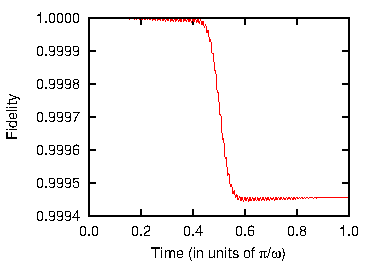
\includegraphics[width=75mm]{Images/HighFreq.pdf}}
    \qquad
    \subfloat[][\label{fig:LowFreq}]{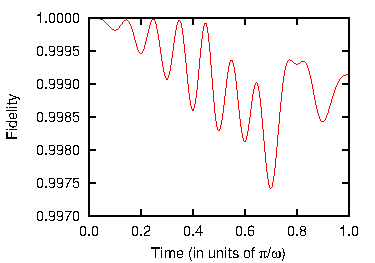
\includegraphics[width=75mm]{Images/LowFreq.pdf}}
    \caption{\label{fig:Fidelity} Fidelities of the wavefunction in
      the presence of a single gravitational wave at different
      frequencies to the unaffected state. \subref{fig:HighFreq}
      $\Omega = 100\omega$. The large drop at $t=\pi/\omega$ is
      evidence that interaction enhances the effect of the
      gravitational waves. \subref{fig:LowFreq} $\Omega =
      10\omega$. We see no evidence of interaction at $t=\pi/\omega$
      as it has no effect in this regime. }
  \end{center}
\end{figure}

We can distinguish two regimes for gravitational waves interacting
with a two particle quantum system in a harmonic trap based on their
relation to the interaction time, $\tau$, which is the length of time
during which the wave packets overlap is significant. Firstly, there
are high frequency waves for which $\Omega \gg \tau^{-1}$. Figure
\ref{fig:HighFreq} shows the evolution of fidelity over a single
collision for a single wave of frequency $\Omega = 100 \omega$. The
biggest change in fidelity occurs during the collision itself when the
wave packets overlap, interact and entangle. Outside the collision,
when the overlap is small the fidelity simply oscillates with an
amplitude that increases with the particle's speed. We clearly see
that the effect of the gravitational wave is amplified in the
interaction which leads to a permanent change in the value of
$\mathcal{F}$. The change in fidelity is dominated by the change in
the entanglement of the two particles due to the radiation. The low
frequency regime is defined as $\Omega \ll \tau^{-1}$. Figure
\ref{fig:LowFreq} clearly shows that such waves have a larger effect
on the fidelity, but it is independent of the interaction. This effect
is classical and the low fidelity is due to a change of the classical
trajectory and final position of the particle in the harmonic
potential. We will not consider low frequency waves in this
investigation anymore since if we were intending on studying such
waves we would not need to resort to a quantum mechanical model to
describe their effect on the particles.

We see from figure \ref{fig:Freqs} that the high frequency regime
begins beyond $10 \omega$ as the inter-particle interaction starts
having a visible effect on the fidelity of the final state. These
results show that entanglement may be more useful in detecting high
frequency gravitational waves rather than a general stochastic
background since the effect of lower frequencies, which affect the
classical behaviour of the system, are much larger. Figure
\ref{fig:Freqs} shows that in the high frequency regime the quantum
effect of the waves on the fidelity can be even $10^6$ larger than the
effect due to the change in the classical trajectory. This
amplification is likely to be even stronger for higher frequencies
when we would no longer be able to ignore the first derivative terms
in equation \eqref{eq:laplacian}. Unfortunately, the gravitational
wave background is predicted not to have any significant components
above \mbox{100 kHz}, which will usually be smaller than or comparable
to the value of $\omega$ for a multilayer trap. Therefore,
entanglement is not a very useful mechanism for detecting background
radiation.

\begin{figure}[htbp]
  \begin{center}
    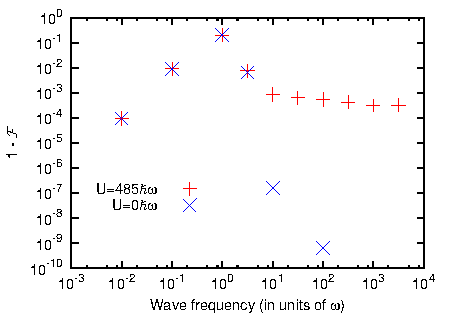
\includegraphics[width=120mm]{Images/Freqs.pdf}
    \caption{\label{fig:Freqs} The fidelity change of the wavefunction
      in the presence of a single gravitational wave to an unaffected
      state for two different interaction strengths. We observe
      resonance at $\omega$ which is in the classical low frequency
      regime. The interplay between the gravitational waves and
      entanglement begins beyond $\Omega = 10 \hbar \omega$.}
  \end{center}
\end{figure}

Figure \ref{fig:EntanglementSingle} shows the von Neumann entropy of
entanglement for a single collision. The form of the entropy does not
change at all as a function of gravitational radiation. However, its
final value does vary in the presence of waves, but the effect is very
small compared to the change due to the particle dynamics in the
collision itself. In the high frequency regime the waves' effect on
the entanglement is larger than their effect on the trajectories of
the particles, therefore, the fidelity of the final state to the
unaffected wavefunction is a better measure of the change in
entanglement of the system than entropy itself.

\begin{figure}[htbp]
  \begin{center}
    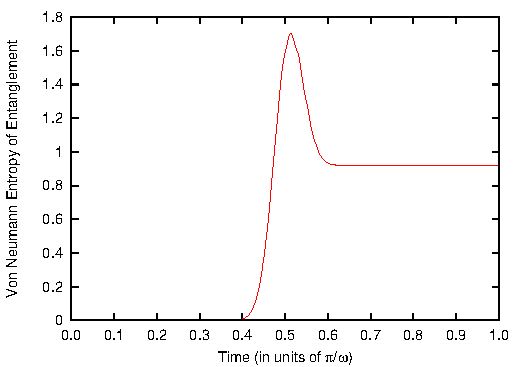
\includegraphics[width=120mm]{Images/EntanglementSingleWave.pdf}
    \caption{\label{fig:EntanglementSingle} The von Neumann entropy of
      entanglement of the wavefunction in the presence of a single
      gravitational wave. Oscillations are present, but they are
      significantly smaller than the change in entropy due to the
      interaction.}
  \end{center}
\end{figure}

The values of the $S$ and $\mathcal{F}$ are plotted over a suitable
range of interaction strengths in figure \ref{fig:Uplot} for a single
high frequency wave. Whilst the largest change in fidelity does not
coincide with the case where the final state is maximally entangled,
the fidelity changes the most when entanglement is produced. This
suggests that the amplification of the effect is due to the wave's
influence on the system's entanglement. Following the fidelity and von
Neumann entropy for multiple collisions confirms the correlation
between fidelity and entropy. The dynamics of particles will cause the
entanglement to increase and decrease during the collisions and the
change in fidelity follows the same trend.

\begin{figure}[htbp]
  \begin{center}
    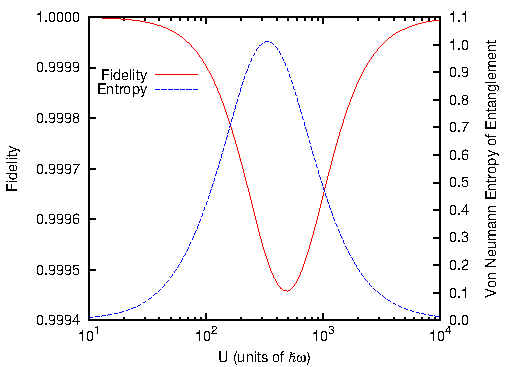
\includegraphics[width=120mm]{Images/Uplot.pdf}
    \caption{\label{fig:Uplot} The values of the von Neumann entropy
      of entanglement and fidelity of the state affected by waves to
      the unaffected state after a single collision. Entanglement
      amplifies the effect of the gravitational wave on the
      wavefunction, but the maximum value of entropy does not coincide
      with the minimum value of fidelity.}
  \end{center}
\end{figure}

To compare the effects of different radiation strengths on the quantum
state we define the intensity of the signal to be $I = \sum_j
(A^{xx}_j)^2$ which is proportional to the energy flux of the wave
\cite{hobson}. All of the results produced so far were calculated for
the largest possible value, $I = 0.01$. Higher intensities are not
investigated since in those cases the weak field approximation is no
longer valid. However, simulating realistic values of strain is beyond
even machine double precision. In order to estimate the size of the
effect of gravitational waves on the quantum state the value of
fidelity is evaluated for different intensities that are within
machine precision. The results in figure \ref{fig:WaveMags} show that
the change in the final value of fidelity is proportional to the
intensity of the waves. This is a very useful relationship as it lets
us easily estimate the size of the gravitational waves' effect for
different intensities. The square of the fidelity $\mathcal{F}^2$ is
just the probability of observing the final state to be that predicted
for a flat spacetime. Therefore, if we measure the final state
(e.g. by measuring the spin of outgoing neutrons) several times then
on average $1 - \mathcal{F}^2$ of the time we should obtain a
different result than predicted by the dynamics of the particles alone
in the absence of radiation. From the results in figure
\ref{fig:WaveMags} we find that $1 - \mathcal{F} = 0.5I$. Therefore,
the probability, $p$, of measuring a different state than expected can
be shown to be
\begin{equation}\label{eq:prob}
p = 1 - \mathcal{F}^2 \approx I.
\end{equation}
Different wave combinations will lead to different numerical
prefactors as the relationship between $1 - \mathcal{F}$ and $I$ is
linear regardless of the frequency regime and number of waves. The
highest intensity we can investigate in the weak field limit and high
frequency regime gives $p=0.01$. This is a small value, but
potentially measurable. However, extrapolating to the expected
detectable values of strain gives $p \approx 10^{-40}$. Assuming
Poissonian statistics in the spin counting process this requires
$\sim10^{27}$ measurements in order to make the error smaller than the
signal which shows that such an experiment is impractical.

\begin{figure}[htbp]
  \begin{center}
    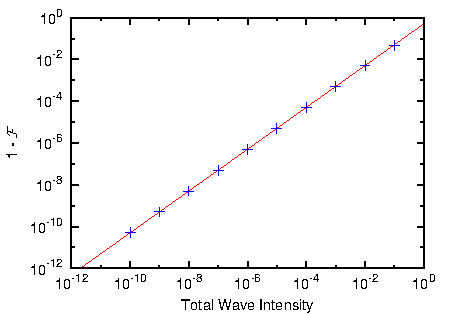
\includegraphics[width=120mm]{Images/WaveMags.pdf}
    \caption{\label{fig:WaveMags} The change in fidelity $\Delta = 1 -
      \mathcal{F}$ plotted against the total intensity. This change is
      proportional to the total intensity $\Delta = 0.5I$ over a very
      large range of values. The relationship is linear regardless of
      the number of waves or the frequency components present. }
  \end{center}
\end{figure}

We can now answer the question whether gravitational waves can be
detected using neutrons in the suggested experiment. We have already
discussed the applicability of the proposed scheme to detecting the
gravitational wave background and concluded that the experiment's
frequency range is too high and the classical effect of low frequency
waves is much larger anyway. We have also shown that the probability
of measuring an effect due to gravitational waves scales linearly with
the wave intensity which means that for realistic wave amplitude
values we will observe a different state only $\sim 10^{-40}$ of the
time. Additionally, it can be shown that for typical multilayer
dimensions and potentials the value of the neutron interaction in
\eqref{eq:nn} will be $U \approx 10^7 \hbar\omega$ which corresponds
to a point beyond the plotted range in figure \ref{fig:Uplot}. This
means that two neutrons introduced in coherent states on either side
of the well will not entangle in the collision and hence the quantum
effect of even high frequency gravitational waves will be minimal. The
neutrons will simply bounce of each other and behave classically. The
most significant effect the waves have on such a system is to cause
the physical separation of the two particles to oscillate and in this
case two neutrons in a multilayer are not the most optimal system for
detecting gravitational waves.

